
 
%%%%%%%%%%%%%%%%%%%%%%%%%%%%%%%%%%%%%%%%%%%%
\section{Effort-Based Incentive Mechanism}
\label{sec__incentives_design}

To ensure sustainability and growth of the community cloud, 
incentive mechanisms are needed that encourage members 
to contribute with their hardware, effort and time. 
When designing such mechanisms, the heterogeneity of the nodes and communication links has to be considered since each member brings in a widely varying set of resources and physical capacity to the system.
Most peer-to-peer (P2P) systems implement incentive mechanisms based on contribution, 
where nodes are rewarded according to resources they donate to the system~\cite{Shen2010}.
We suggest an effort-based incentive mechanism for community cloud, 
where effort is defined as contribution relative to the capacity of a node~\cite{Khan2015Incentive}. 
This mechanism is inspired by the \emph{Parecon} economic model~\cite{Albert2004Parecon, Rahman2010, Vega2013Sharing}, 
which focuses on social welfare by considering inequality among nodes. 
Nodes with different capacity cannot have same contribution to the system, 
but with effort-based mechanism they get same reward if they share as much as possible of their capacity, 
as we explain in \Cref{sec__incentive_formulations}.
We can use a system of credits, acting as virtual currency, 
to facilitate transactions between providers and consumers.
When resources are consumed, providers earn credits which they can later use to request resources from the system.
We assume, because of the trust among the community, that users truthfully report the capacities of their nodes.

%%%%%%%%%%%%%%%%%%%%%%%%%%%%%%%%%%%%%%%%%%%%
\subsection{Formulations}
\label{sec__incentive_formulations}
% Calculation of Transaction Cost and Credits

We first discuss the criteria that a SN uses to evaluate requests from ONs.
When a node asks for a resource from a SN, which in this case means to commit an instance of VM for a given duration, the SN first checks whether the ON's credit is sufficient to cover the cost of the transaction.
The cost given in \cref{eq__transaction_cost} is proportional to the number of resources requested ${ R }_{ i }$ and the duration ${ T }_{ i }$ for how long they are required.
The nonzero coefficients $\gamma$ and $\rho$ apply to the amount and duration of resources shared respectively, 
and provide a way to tweak the value generated by the transactions, 
which is useful to control the behaviour when implementing the prototype system.

\begin{equation}
	\text{\emph{transaction\_cost}} = \gamma { R }_{ i } \times \rho { T }_{ i }
	\label{eq__transaction_cost}
\end{equation}

The cost from all the past transactions node $i$ participates in, either as a provider or a consumer, determines the level of its credit. 
SN keeps track of the history of all the past transactions, and the credit of each node.
If the requesting node does not have enough credit, the request is rejected. 
Otherwise, the SN searches for nodes that have resources available. 
It selects as many nodes as possible from its local zone to provide the resources.
If the demand cannot be met locally, the SN forwards the request to other SNs in the federated community cloud.

Now we consider how the SN manages the credits of the nodes that take part in the transaction.
For each node which contributes its resources to fulfil the request, the SN calculates the transaction cost from \cref{eq__transaction_cost}, and adds it to that node's credits. 
The cost is deducted from the credits of the node that consumed the resources.
After the transaction is completed, the effort for each node involved in the transaction is recalculated using \cref{eq__credit}.
Here ${credit}_{i}$ represents the total credit of the node $i$, 
taking into account the outcome of the most recent transaction.
The nonzero coefficient $\epsilon$ applies to the capacity of the node,
and acts as a normalising factor taking into account the overall capacity in the system.
A selfish node not contributing enough has effort ${ E }_{ i } < 1$, 
and will be at a disadvantage when requesting resources, 
as in \cref{eq__node_requested_resources}.

%% Notes on package conflicts with following equation:
%%  Do not enable following packages, will produce errors in compilation:
%%		\usepackage{mdwmath}
%%		\usepackage{mdwtab}
%% Do use the following packages, otherwise you will get errors:
%%		\usepackage[cmex10]{amsmath}
\begin{equation}
    \begin{IEEEeqnarraybox}{rCl} % Note the equation uses IEEEeqnarray, so need to include \usepackage{IEEEtrantools}
        { E }_{ i }\quad = 
        \begin{cases}
            \frac{{\text{\emph{credit}}}_{i}}{ \epsilon {C}_{i}} \quad if \quad \frac{{\text{\emph{credit}}}_{i}}{ \epsilon {C}_{i}} < 1 \quad \\
            \quad 1  \qquad \text{\emph{otherwise}}
        \end{cases}    
    \end{IEEEeqnarraybox}
    \label{eq__credit}
\end{equation}

The effort ${ E }_{ i }$ of a node expresses its relative contribution to the system, 
since the mechanism considers the capacity ${ C }_{ i }$ of a node as well. 
This means that a node with low capacity puts in more effort than a node with high capacity even if both of them donate same amount of resources to the system.
For total $N$ nodes in the system, the total amount of available resources ${\Omega}$ is the sum of the resources ${ { \omega } }_{ i }$ contributed by each node $i \in N$ (out of its total capacity ${ C }_{ i }$).

%% EQUATION
\begin{equation}
	\Omega =  \sum_{i \in N}{ { \omega  }_{ i } }
	\label{eq__total_resources}
\end{equation}

The maximum resources node $i$ can consume, ${ { \Delta R } }_{ i }$, depends upon its effort ${ E }_{ i }$.
A node actively contributing to the system has ${ E }_{ i } = 1$, and so can access all the available resources ($\Omega - { \omega  }_{ i }$), but a selfish node with ${ E }_{ i } < 1$ gets penalised with limited access to the resources.

%% EQUATION
\begin{equation}
	{ \Delta R }_{ i } ={ E }_{ i } \times ( \Omega - { \omega  }_{ i })
	\label{eq__node_requested_resources}
\end{equation}

The effort-based mechanism implies that the nodes with better resources may find it beneficial to under-report their capacity in some cases. 
This requires that the mechanism should be carefully designed so as not to penalise high capacity nodes too much. 
Moreover, within a community of trusted users, we assume that the social context encourage users to be truthful when reporting the capacity to SN, 
and that the community may employ other mechanisms to verify the capacity of the nodes.

%%%%%%%%%%%%%%%%%%%%%%%%%%%%%%%%%%%%%%%%%%%%%
\subsection{Algorithm for Requests Processing}

%%% FIGURE
\begin{figure}[tbp]
	\centering
	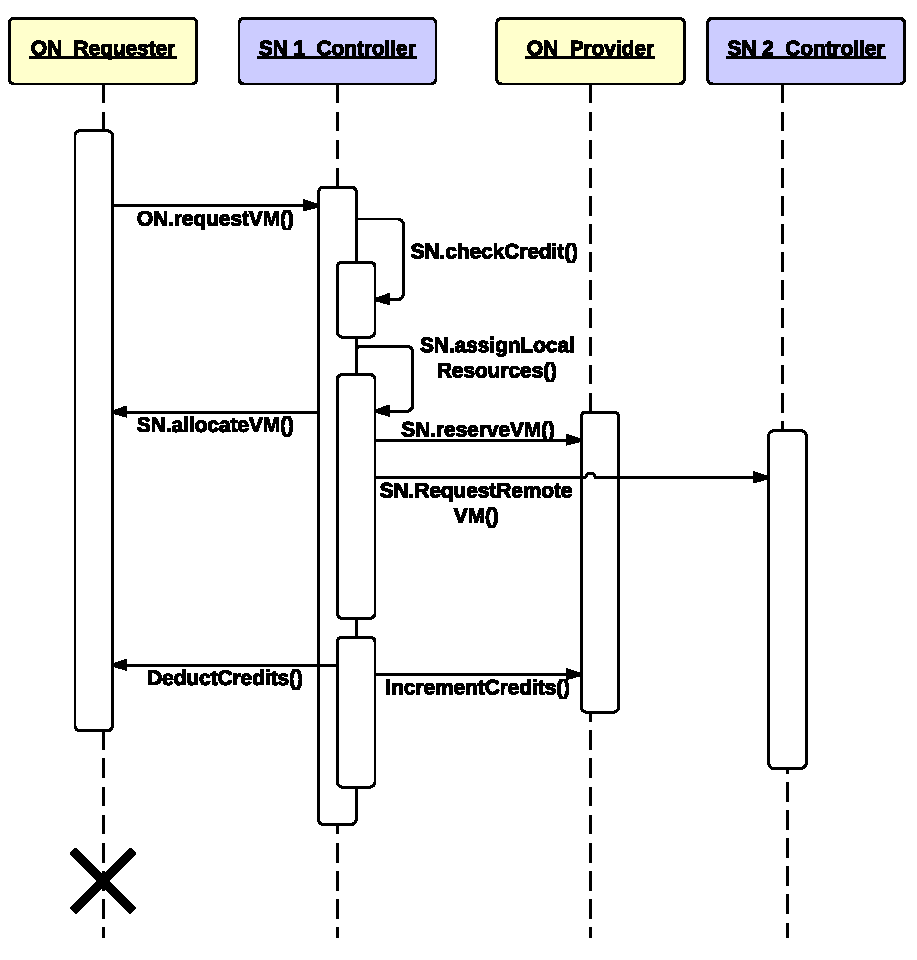
\includegraphics[width=0.55\textwidth,keepaspectratio]{SNSequenceDiagram}
	\caption{Details of the VM request operation by ON}
	\label{fig:sequence-dig-controller-request}
\end{figure}

Algorithm~\ref{fig__incentives_algo_request_processing} explains how a SN handles request from a node in its zone.
When SN receives a request, it first calculates that node's allowance $\Delta {R }_{ i }$ to confirm whether it has enough credit to fulfil the request. 
If not, the request is rejected, otherwise the algorithm calls \textsc{decision} function which searches for available resources (lines 1--5).
The \textsc{decision} function first checks if enough resources are available in the local zone (line 8), 
and selects the nodes that will provide the resources from its local zone (line 9).
If SN cannot satisfy request from its local nodes, it forwards request to one of its neighbouring SNs (lines 16--18).
After the provider nodes commit resources, SN calculates cost of the transaction and updates the 
nodes' credits, deducting credits from the requester and increasing credits of the providers (lines 10--14).
The sequence of steps is depicted in Figure~\ref{fig:sequence-dig-controller-request}.


%%%%%%%%%%%%%%%%%%%%%%
\begin{algorithm}[tbp]
	\small
	\begin{algorithmic}[1]

		\Require{receive query from node \emph{i} with the requested amount ${ R }_{ i }$ and the time ${ T }_{ i }$ }

		\State calculate ($\Delta { R }_{ i }$)
		
		\If{${ { R }_{ i } <= \Delta R }_{ i } $}
		\State call \textsc{Decision} (\emph{i},\,${ R }_{ i }$,\,${ T }_{ i }$)
		\Else
		\State send (``rejected'',\,\emph{i})
		\EndIf

		%% \State \textbf{function} DECISION(${i}$, ${ R }_{ i }$, ${ T }_{ i }$)
		\Procedure{Decision } {${i}$, ${ R }_{ i }$, ${ T }_{ i }$}
		\If{${R}_{ i } <= \Omega$}
		\State \emph{ProvidersList}[n]  $\leftarrow$ provider (\emph{ON\_List},\,${ R }_{ i }$)
		\For{\textbf{each} j in \emph{ProviderList}[n]}
		\State ${\text{\emph{Cost\,Of\,Transaction}}}_{j \rightarrow i} \leftarrow {R}_{ j }^{ r} * {T }_{ j }^{t}$
		\State update\_credits (${\text{\emph{Cost\,Of\,Transaction}}}_{j \rightarrow i}$) 
		\State update\_database (\emph{ON\_List})
		\EndFor
		\Else
		\State \emph{SN} $\leftarrow$ provider (\emph{SN\_List},\,${ R }_{ i }$) 
		\State forward (\emph{SN},\,\emph{i},\,${ R }_{ i }$,\,${ T }_{ i }$)
		\EndIf
		\EndProcedure

	\end{algorithmic}
	\caption{Handling requests from ONs}
	\label{fig__incentives_algo_request_processing}
\end{algorithm}
%%%%%%%%%%%%%%%%%%%%%%

If the request from an ON is rejected, ON can submit the request again to SN after some time.
In the current implementation, resources are assigned to whoever first requests them as they become available. 
So this may not be fair in the sense that the time users have been waiting for the resources is not taken into account.
This issue can be addressed by using queuing at the SN to keep track of the pending requests.
Similarly, a related issue occurs when there may be multiple ONs that the SN can pick as providers for a given request.
Therefore, SN may have to apply a selection mechanism for prioritising which ONs to choose as providers. 
We have studied the effect of some selection mechanisms 
on the performance in~\cite{Khan2013TowardsIncentives}, 
and we leave further investigation of these issues for future work.
